





\documentclass[
% handout
serif,
mathsans,
]
{beamer}
\usepackage[utf8]{inputenc}
% \usetheme[width=6ex]{Marburg}
% \usetheme[width=6ex]{Goettingen}
\usetheme[height=1cm]{Rochester}
\useinnertheme{circles}
% \useoutertheme[compress,subsection=false]{miniframes}
\usecolortheme{rose}
 \setbeamertemplate{navigation symbols}{}
\usepackage[T1]{fontenc}

\usepackage{csquotes}	



\usepackage{verbatim}
\usepackage{tikz}
\usetikzlibrary{shapes}                
\usetikzlibrary{fit}

% \renewcommand*\ttdefault{lmvtt}
% \renewcommand*\familydefault{\ttdefault} %% Only if the base font of the document is to be typewriter style


% \RequirePackage{emerald}
% \usepackage{comicsans}
% \usepackage{winfonts}

%\usepackage{pdfpages}
\usepackage{graphicx}

\usepackage{amsmath, amsthm}
% \usepackage{amssymb}
% \usepackage{ascii}
%  \usepackage{tikz}

 \RequirePackage{xcolor}
\RequirePackage[color,all,2cell]{xy}\SelectTips{cm}{12}\SilentMatrices\UseAllTwocells  % commutative diagrams

\usepackage{bussproofs}

\definecolor{dkblue}{rgb}{0,0.1,0.5}
\definecolor{lightblue}{rgb}{0,0.5,0.5}
\definecolor{dkgreen}{rgb}{0,0.4,0}
\definecolor{dk2green}{rgb}{0.4,0,0}
\definecolor{dkviolet}{rgb}{0.6,0,0.8}

% \usepackage{arev}
\usepackage{listings}
\newcommand{\sss}{\ttfamily\bfseries\small}
\def\lstlanguagefiles{defManSSR.tex}\lstset{language=SSR}

% \usepackage[bitstream-charter]{mathdesign}
%  \usepackage{palatino}\linespread{1.05}
% \usepackage{verbatim}

\title[Coinitial semantics for redecoration]{Coinitial semantics \\ for redecoration of triangular matrices}
\author{Benedikt Ahrens and R\'egis Spadotti}
% \date{2011--09--11}
% \date{Sept 11, 2011}
\date[put date here]{Conference on stuff}
%{19th Workshop on \\ Logic, Language,  Information and Computation}

\institute[IRIT] % (optional, but mostly needed)
{%
%   Centre International de Math\'ematique et Informatique de Toulouse\\
  Institut de Recherche en Informatique de Toulouse\\
   Universit\'e Paul Sabatier\\ ~ \\
%     \includegraphics[height=1em]{logo_irit.jpg} 
%          \hspace{1cm} \includegraphics[height=1em]{logo_ups.jpg}
%   Equipe ACADIE
}

\setbeamertemplate{footline}
{%
  \leavevmode%
  \hbox{\begin{beamercolorbox}[wd=.5\paperwidth,ht=2.5ex,dp=1.125ex,leftskip=.3cm plus1fill,rightskip=.3cm]{author in head/foot}%
    \usebeamerfont{author in head/foot}\insertshortauthor
  \end{beamercolorbox}%
  \begin{beamercolorbox}[wd=.5\paperwidth,ht=2.5ex,dp=1.125ex,leftskip=.3cm,rightskip=.3cm plus1fil]{title in head/foot}%
    \usebeamerfont{title in head/foot}\insertshorttitle\hfill\insertframenumber/\inserttotalframenumber
  \end{beamercolorbox}}%
  \vskip0pt%
}

\newcommand{\constfont}[1]{\ensuremath{\mathsf{#1}}}

\newcommand{\C}{\mathcal{C}}
\newcommand{\D}{\mathcal{D}}
\newcommand{\N}{\mathbb{N}}
\newcommand{\bind}[2]{{#1}\mathbin{\gg\hspace{-.8ex}=}{#2}}
\newcommand{\Tri}{\constfont{Tri}}
\newcommand{\head}{\constfont{top}}
\newcommand{\tail}{\constfont{rest}}
\newcommand{\bisim}{\constfont{bisim}}
\newcommand{\redec}{\constfont{redec}}
\newcommand{\cut}{\constfont{cut}}
\newcommand{\ccut}{\constfont{ccut}}
\newcommand{\RComonad}{\constfont{RComonad}}
\newcommand{\RComonadWC}{\constfont{\RComonad wCut}}
\newcommand{\ULCop}{\constfont{LC}}
\newcommand{\induced}[1]{\ensuremath{\langle {#1} \rangle}}

\newcommand{\shift}{\constfont{shift}}
\newcommand{\lift}{\constfont{lift}}
\newcommand{\abs}{\constfont{abs}}
\newcommand{\subst}{\constfont{subst}}
\newcommand{\Setoid}{\constfont{Setoid}}
\newcommand{\eq}{\ensuremath{\mathsf{eq}}}

\newcommand{\coq}{\texttt{Coq}\xspace}

%  \newcommand{\bind}[2]{{#1} \blacktriangleright {#2}}
% \newcommand{\bind}[2]{{#1} \mathbin{\vartriangleright} {#2}}
% \newcommand{\bind}[2]{{#1} \mathbin{\mathbf{\rhd}} {#2}}
\newcommand{\TLCar}{\Rightarrow}
\newcommand{\TS}[1]{Set^{#1}}
\newcommand{\fibre}[2]{\ensuremath{{#1}[{#2}]}}
\newcommand{\LC}{\mathsf{LC}}
\newcommand{\TLC}{\mathsf{TLC}}
\newcommand{\PCF}{\mathsf{PCF}}

\newcommand{\Id}{\mathsf{Id}}


\newcommand{\Set}{\mathsf{Set}}
\newcommand{\PreOrd}{\mathsf{Pre}}

\newcommand{\PCFar}{\Rightarrow}
\newcommand{\Bool}{Bool}
\newcommand{\Nat}{Nat}

\DeclareMathOperator{\dom}{dom}
\DeclareMathOperator{\cod}{cod}

\newcommand{\init}[1]{\hat{#1}}
\newcommand{\retyping}[1]{\vec{#1}}

\newcommand{\fat}[1]{\textbf{#1}}

\AtBeginSection[]
 {
    \begin{frame}
        \frametitle{Outline}
        \tableofcontents[currentsection]
    \end{frame}
 }


\begin{document}

\begin{frame}
\titlepage

\end{frame}

\section{Initiality for W-types and heterogeneous inductives}

\begin{frame}
 \frametitle{Starting point: W-types in categories}
 
 \begin{block}{Well-founded trees as initial algebra of polynomial functor}
  \begin{itemize}
   \item Dybjer '97, Moerdijk and Palmgren '00
  \end{itemize}
 \end{block}

 \begin{block}{Extended to some \fat{heterogeneous} data types}
 
  \begin{itemize}
    \item Fiore, Plotkin, Turi '99, Hirschowitz and Maggesi '07
    \item motivation: characterization of \fat{binding signatures} (e.g.\ $\lambda$-calculus)
    \item binding modelled through \fat{heterogeneous} data type
           \[  \lambda : \LC(X + 1) \to \LC(X) \]
    \item characterizes not only data, but also \fat{substitution} operation
%    \begin{itemize}
%     \item 
  \end{itemize}
%     \item variant using monads: Altenkirch \& Reus '99, Hirschowitz \& Maggesi '07, '10
%    \end{itemize}
 \end{block} 
\end{frame}

\begin{frame}
 \frametitle{Overview over work by Hirschowitz and Maggesi '07}
 \begin{block}{Builds upon Altenkirch and Reus '99}
  \begin{itemize}
   \item Lambda calculus as heterogeneous data type
   \item Lambda calculus \fat{+ substitution} forms a \fat{monad}
  \end{itemize}
 \end{block}

\begin{block}{Hirschowitz and Maggesi '07}
 \begin{itemize}
  \item Lambda calculus as \fat{inital} monad 
     \begin{itemize}
       \item [$\leadsto$]actually: monad + extra structure for constructors
     \end{itemize}
  \item notion of \fat{module over a monad} 
     \begin{itemize}
        \item [$\leadsto$]used to characterize constructors of lambda calculus
     \end{itemize}
 \end{itemize}
\end{block}
\end{frame}


\begin{frame}
 \frametitle{Goal: characterize \fat{co}data types with \fat{co}substitution}
 
\begin{block}{Question}
  \begin{itemize}
    \item 
        Can we use (dual) techniques of H.\ and M.\ to characterize codata types with cosubstitution as
        \fat{terminal} object?
    \item I.e.: Given some codata type, what is the category in which that codata type is terminal?
  \end{itemize}
\end{block}
  
\begin{block}{In this talk}
 we answer this question for 
  \begin{itemize} 
    \item the codata type of infinite triangular matrices
    \item with \fat{redecoration} operation
  \end{itemize}
\end{block}

 
\end{frame}


\begin{comment}
\begin{frame}
 \frametitle{Binding signatures with (in)equations}
   \begin{block}{Equational theories}
    \begin{itemize}
     \item prime example: lambda calculus modulo $\beta$-equivalence
     \item Fiore with students Hur \& Mahmoud
     \item Hirschowitz \& Maggesi %TODO: which paper?
    \end{itemize}
   \end{block}
   
  \begin{block}{Reduction rules via \fat{in}equations}
   \begin{itemize}
    \item A., PhD thesis: 
     \begin{itemize}
      \item based on ideas by Hirschowitz \& Maggesi
      \item uses notion of \fat{relative} monad (Altenkirch et al. '10)
     \end{itemize}
   \end{itemize}
  \end{block}
  
  \begin{block}{Goal:}
   do the same for cosyntax, i.e.\ \fat{nested co}data types %TODO: explain cosyntax
  \end{block}
\end{frame}
\end{comment}

\section{Cosyntax: infinite triangular matrices and redecoration}

\begin{frame}
 \frametitle{An example of cosyntax: infinite triangular matrices}
 
   \begin{block}{\Tri: the codata type of infinite triangular matrices}
     \begin{itemize}
      \item omit redundant information below the diagonal
      \item have a \fat{variable} type $A$ of diagonal elements 
        \begin{itemize} 
          \item e.g.\ invertible elements
        \end{itemize}
      \item a fixed type $E$ of elements for rest of matrix
      \item usage: Pascal matrices (binomial coefficients), mathematical physics (infinite-dim.\ problems)
     \end{itemize}
   \end{block}
   
   
\begin{center}
   
 
%
  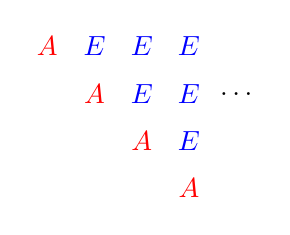
\begin{tikzpicture}[scale = 0.6]
     \foreach \y in {0,...,2}
     {\foreach \x in {\y,...,2}
       \draw (\x+1, -\y) node[color=blue]{$E$} ;
     }
     \foreach \x in {0,...,3} \draw (\x, -\x) node[color=red]{$A$} ;
     \draw(4,-1) node{$\ldots$};
%      \draw[style = dashed](0.5,0.2) -- (0.5,-1.2);
%      \draw[style = dashed](1.5,0.2) -- (1.5,-2.2);
%      \draw[style = dashed, thin](2.5,0.2) -- (2.5,-3.2);
     
%      \draw[color=green]  (3,0.5) -- (0.3,0.5) -- (0.3,
%      -1.2)  -- (2.8,-3.6);
%      \draw[color=green, dashed]  (3,0.5) -- (4,0.5);
%      \draw[color=green, dashed]  (2.8,-3.6) -- (3.5,-4.2);
 \end{tikzpicture}

\end{center}
 

   
\end{frame}

\begin{frame}
 \frametitle{Matrices through trapezes: the destructors of TriMat}
 
 
 
\begin{columns}

 \column{.4\textwidth}
 
 \begin{center}
 
  \def\proofSkipAmount{\vskip.8ex plus.8ex minus.4ex}
    \AxiomC{$t : \Tri(A)$}\doubleLine
     \UnaryInfC{$\head_A(t) : A$}
      \DisplayProof
                      
 
 \vspace{15ex}
 
  \AxiomC{$t : \Tri(A)$}\doubleLine
                                       \UnaryInfC{$\tail_A(t) : \Tri(E\times A)$}
                                       \DisplayProof%
 
 \end{center}
 
 \vspace{5ex}
 
 \column{.5\textwidth}

\vspace{2em}
 
  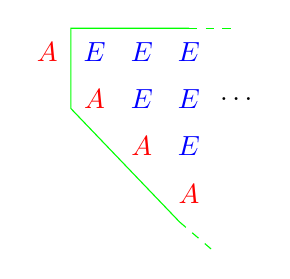
\begin{tikzpicture}[scale = 0.6]
     \foreach \y in {0,...,2}
     {\foreach \x in {\y,...,2}
       \draw (\x+1, -\y) node[color=blue]{$E$} ;
     }
     \foreach \x in {0,...,3} \draw (\x, -\x) node[color=red]{$A$} ;
     \draw(4,-1) node{$\ldots$};
%      \draw[style = dashed](0.5,0.2) -- (0.5,-1.2);
%      \draw[style = dashed](1.5,0.2) -- (1.5,-2.2);
%      \draw[style = dashed, thin](2.5,0.2) -- (2.5,-3.2);
     
     \draw[color=green]  (3,0.5) -- (0.5,0.5) -- (0.5,
     -1.2)  -- (2.8,-3.6);
     \draw[color=green, dashed]  (3,0.5) -- (4,0.5);
     \draw[color=green, dashed]  (2.8,-3.6) -- (3.5,-4.2);
 \end{tikzpicture}
 
\vspace{5ex}
 
  \begin{overprint}
    \onslide<2>
\hspace{1em}    
	  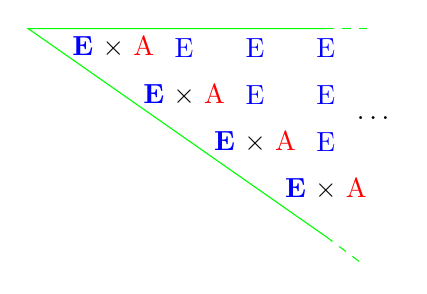
\begin{tikzpicture}[scale = 0.6]
	  \foreach \y in {0,...,2}
	    {\foreach \x in {\y,...,2}
	      \draw (1.5*\x+10.5, -\y) node[color=blue]{E} ;
	    }
	    \foreach \x in {0,...,3} \draw (1.5*\x+9, -\x)
	    node{{\color{blue}\textbf{E}} $\times$ {\color{red} A}} ;
	    \draw(14.5,-1.5) node{$\ldots$};
	    
	    \draw[color=green] (13.5,0.4) -- (7.2,0.4) -- (13.5, -4); 
	    \draw[color=green, dashed] (13.5,0.4) -- (14.4,0.4) ; 
	    \draw[color=green, dashed] (13.5,-4) -- (14.3,-4.6) ; 
	  \end{tikzpicture}
    \onslide<1>
\hspace{1em}
	    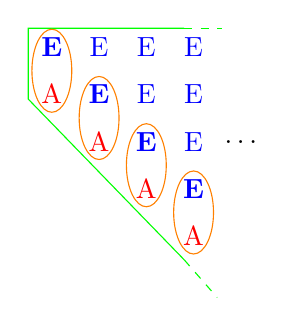
\begin{tikzpicture}[scale = 0.6]
	    % matrix coefficients
	    \foreach \y in {0,...,2}
	    {\foreach \x in {\y,...,2}
	      \draw (\x+1, -\y) node[color=blue]{E} ;
	    }
	    \foreach \x in {0,...,3} \draw (\x, -\x-1) node[color=red]{A} ;
	    \foreach \x in {0,...,3} \draw (\x, -\x)
	    node[color=blue]{\textbf{E}} ;
	    \draw(4,-2) node{$\ldots$};
	    
	    % green border
	    \draw[color=green] (2.8,0.4) -- (-0.5,0.4) -- (-0.5, -1.1) --
	    (2.8,-4.5)  ; 
	    \draw[color=green, dashed] (2.8,0.4) -- (3.6,0.4) ; 
	    \draw[color=green, dashed] (2.8,-4.5) -- (3.5,-5.3) ; 
	    
	    % ellipses around pairs of A and E
	    \draw[color=orange](0, -0.5) ellipse (12pt and 25pt) ;  
	    \draw[color=orange](1, -1.5) ellipse (12pt and 25pt) ;  
	    \draw[color=orange](2, -2.5) ellipse (12pt and 25pt) ;  
	    \draw[color=orange](3, -3.5) ellipse (12pt and 25pt) ;  
	  \end{tikzpicture}
  \end{overprint}
 
 
  \end{columns}
\end{frame}  


  
 

\begin{frame}
 \frametitle{Redecoration}
 
 
 \[\redec_{A,B} : (\Tri A \to B) \to (\Tri A \to \Tri B) \]
 \centering
 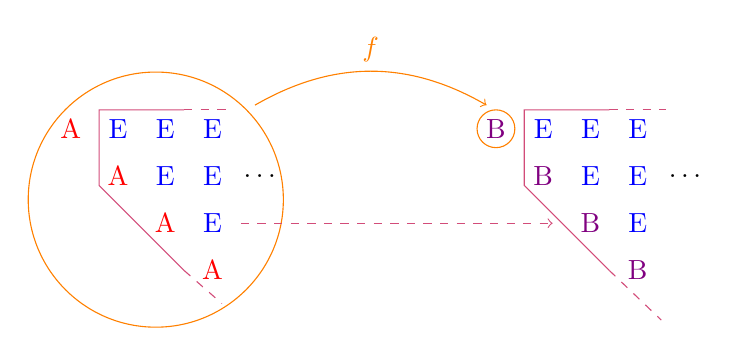
\begin{tikzpicture}[scale = 0.6]
    \foreach \y in {0,...,2}
    {\foreach \x in {\y,...,2}
      \draw (\x+1, -\y) node[color=blue]{E} ;
    }
    \foreach \x in {0,...,3} \draw (\x, -\x) node[color=red]{A} ;
    \draw(4,-1) node{$\ldots$};

    \foreach \y in {0,...,2}
    {\foreach \x in {\y,...,2}
      \draw (\x+10, -\y) node[color=blue]{E} ;
    }
    \foreach \x in {0,...,3} \draw (\x+9, -\x) node[color=violet]{B} ;
    \draw(13,-1) node{$\ldots$};
    \draw[color=purple!70]  (2.4, -3) --
    (0.6,-1.2) -- (0.6,0.4) -- (2.4,0.4);
    \draw[color=purple!70, dashed]  (2.4,0.4) -- (3.4,0.4);
    \draw[color=purple!70, dashed]  (2.4,-3) -- (3.2,-3.7);
 
    \draw[color=orange] (1.8,-1.5) circle(2.7cm);

    \draw[color=purple!70]  (11.4, -3) --
    (9.6,-1.2) -- (9.6,0.4) -- (11.4,0.4);
    \draw[color=purple!70, dashed]  (11.4,0.4) -- (12.6,0.4);
    \draw[color=purple!70, dashed]  (11.4,-3) -- (12.5,-4.05);
    
    \draw[color=orange] (9,0) circle(0.4cm);
    
    \draw[->,color = orange] (3.9,0.5) to [bend left] node[auto,
    swap, above]{$f$} (8.8,0.5) ; 

    \draw[->,color = purple!70, dashed] (3.6,-2) to (10.2,-2) ; 
  \end{tikzpicture}
 
 When redecorating the $\tail$ of the matrix, we need a function \[\lift~f : \Tri(E\times A) \to E \times B\]
   
\end{frame}

\begin{frame}
 \frametitle{Sameness for infinite triangular matrices}
  \begin{block}{Sameness = \fat{bisimilarity}}
    Bisimilarity $\sim$ coinductively defined via destructors
     
    \begin{center}
                                            \def\extraVskip{3pt}
     \def\proofSkipAmount{\vskip.8ex plus.8ex minus.4ex}
    \AxiomC{$t \sim t'$}\doubleLine
     \UnaryInfC{$\head(t) = \head(t')$}
      \DisplayProof
                        \hspace{3ex}
                                       \AxiomC{$t \sim t'$}\doubleLine
                                       \UnaryInfC{$ \tail(t) \sim \tail(t')$}
                                       \DisplayProof   
   \end{center}                                    
  \end{block}
  
  \begin{block}{Consequences}
    \begin{itemize}
     \item consider $\Tri A$ as a \fat{setoid} rather than a set
     \item \[ \redec_{A,B} : \Setoid(\Tri A,\eq B) \to \Setoid(\Tri A,\Tri B )\]
             with $\eq : \Set \to \Setoid$
    \end{itemize}
  \end{block}

  
\end{frame}


\section{Algebraic characterization of redecoration}

\begin{frame}
 \frametitle{$\Tri$ as a comonad}
\begin{lemma}[Matthes and Picard '11]
 $\Tri$ forms a \enquote{weak constructive comonad}.
\end{lemma}

\begin{lemma}[Equivalent to MP'11]
 $\Tri$ forms a \fat{relative comonad}, relative to $\eq:\Set\to\Setoid$.
\end{lemma}


\end{frame}


\begin{frame}
 \frametitle{Weak constructive comonad}
 \begin{block}{Monads capture substitution and its properties}
   \begin{itemize}
    \item Lambda calculus as monad: Altenkirch \& Reus '99
   \end{itemize}
 \end{block}

\begin{block}{Dually, comonads capture redecoration}
   \begin{itemize}
    \item finite triangular matrices: comonads
    \item infinite triangular matrices need \fat{bisimilarity}
    \item notion of \enquote{weak constructive comonad} introduced by Matthes \& Picard
   \end{itemize}
\end{block}

 
 
\end{frame}



% \begin{frame}
%  \frametitle{Outline}
%   \tableofcontents
% \end{frame}



\section*{Introduction}


\begin{frame}
 \frametitle{Universal algebra}
 
 \begin{columns}
  
  \column{.45\textwidth}

  \begin{block}{Goal of Universal algebra}
   specify
   \begin{itemize}
    \item terms
    \item equations of terms
   \end{itemize}
   by a signature
  \end{block}

  \begin{exampleblock}{\textbf{Signature} of group theory:}
     \begin{itemize}
      \item $e : 0$
      \item $(\_)^{-1} : 1$
      \item $ * : 2$
      \item [+] equations
     \end{itemize}
  \end{exampleblock}
  
  
   \column{.4\textwidth}
 
 \begin{exampleblock}{A group $G$ is a set $G$ with}
 
    operations and equations:
   \begin{itemize}
    \item $e : G$
    \item $(\_)^{-1} : G \to G$
    \item $(*) : G \times G \to G$
%    \end{itemize}
%    equations:
%    \begin{itemize}
    \item $ e * g = g$
    \item $g * g^{-1} = e$
    \item \ldots
   \end{itemize}

  \end{exampleblock}
  
  \begin{block}{The \textbf{free} group of a set $X$} 
     inductively generated by the signature.
  \end{block}

  
 \end{columns}
 
 
\end{frame}


\begin{frame}
 \frametitle{Goal: Universal algebra for programming languages}
  
   \begin{block}{Goal: signatures for languages \textbf{with variable binding}}
    \begin{itemize}
     \item want \textbf{in}equalities rather than equalities between terms
     \item [$\rightsquigarrow$] model reductions more faithfully
     \item characterize language specified by signature categorically
    \end{itemize}

  \end{block}
  
 \begin{columns}
  
  \column{.45\textwidth}
  \begin{block}{Signatures specifying}
      \begin{itemize}
        \item types + 
                    terms
        \item reduction rules
      \end{itemize}
  \end{block}
  
  \column{.45\textwidth}
  \begin{block}{Characterization of generated language}
      \begin{itemize}
         \item category of \textbf{models} of signature
        \item language as \textbf{initial} model % object in some category of \textbf{models} of that signature
      \end{itemize}
  \end{block}
\end{columns}
\end{frame}


\begin{frame}
 \frametitle{Universal algebra with variable binding: related work}
%   \begin{block}{Related work:}
    \begin{itemize}
     \item Gabbay \& Pitts 
        \begin{itemize}
           \item nominal syntax, no equations
        \end{itemize}
     \item Hofmann, Miculan \& Scagnetto 
          \begin{itemize}
             \item HOAS, no equations
          \end{itemize}
     \item Fiore 
        \begin{itemize}
           \item algebraic de Bruijn, equations
        \end{itemize}
     \item Hirschowitz \& Maggesi
        \begin{itemize}
           \item algebraic de Bruijn, equations
        \end{itemize}
    \end{itemize}
%   \end{block}
  
  \begin{block}{My work}
    \begin{itemize}
     \item inspired by Hirschowitz \& Maggesi
     \item adapted to 
      \begin{itemize}
        \item \textbf{in}equalities
        \item simple typing
      \end{itemize}
    \end{itemize}

  \end{block}

  
\end{frame}


\begin{frame}
 \frametitle{Content of this talk}
  
   \begin{block}{In this talk:}
    \begin{itemize}
     \item \textbf{Models} of the untyped $\lambda$-calculus with $\beta$-reduction
     \item the $\lambda$-calculus as \textbf{initial} such model
    \end{itemize}
   \end{block}

   \begin{block}{\textbf{Not} in this talk --- but elsewhere:}
    \begin{itemize}
     \item General notion of \textbf{signature} for languages with reduction
     \item Signatures and models for \textbf{simply-typed} languages with term reductions
    \end{itemize}
   \end{block}

   First: take a look at H \& M's work on $\lambda$-calculus without reductions
   
\end{frame}

\section{Review of Hirschowitz \& Maggesi's work}

\begin{frame}
 \tableofcontents %[currentsection]
\end{frame}


\begin{frame}[fragile]
 \frametitle{$\lambda$-calculus as a monad on $\Set$ (Altenkirch \& Reus '99)}
 
 \begin{lstlisting}
 Inductive LC (V : Set) : Set := 
    | Var : V -> LC(V)
    | Abs : LC(option V) -> LC(V)
    | App : LC(V) x LC(V) -> LC(V)
\end{lstlisting}
 
 \begin{itemize}
  \item  Monad: set of terms over free variables
        \[ \LC(V) = \text{ set of lambda terms over free variables in set } V \]
  \item Monad structure: ``Variables--as--terms'' and substitution
        \begin{align*} Var_{V} &: V \to \LC(V) \\
                       (\bind{}{})_{V,W} &: \LC(V) \times \bigl(V \to \LC(W)\bigr) \to \LC(W)
        \end{align*}

  \item Monad axioms: properties of variable substitution
 \end{itemize}

 
\end{frame}

\begin{frame}
 \frametitle{Constructors and substitution}
  \begin{block}{Goal: capture the interplay between constructors and substitution}
  \vspace{-1.5em}
    \begin{align*}
\bind{App(M,N)}{f} \enspace &= \enspace App(\bind{M}{f},\bind{N}{f}) \\
\bind{Abs(M)}{f} \enspace &= \enspace Abs \bigl(\bind{M}{\shift{f}}\bigr)
    \end{align*}
  \vspace{-1.5em}
  \end{block}
  
 \begin{block}{First try: are $Abs$ and $App$  \textbf{monad morphisms}?}
  \vspace{-1.5em}
       \begin{align*}
                    Abs &: \LC^* \to \LC \qquad\qquad \text{with } \LC^*:V \mapsto \LC(\text{option }V) \\
                    App &: \LC \times \LC  \to \LC
       \end{align*}
\vspace{-1.5em}

\textbf{Fails:} 
   \begin{itemize} 
      \item $\LC^*$ a monad, but $Abs$ \textbf{not}  monad morphism 
      \item $\LC \times \LC$ not a monad in a reasonable sense
   \end{itemize}

  \end{block}



 
\end{frame}

\begin{frame}
 \frametitle{Modules over monads}
  \begin{block}{\textbf{Modules over monads} generalize monads...}
    and the functors
      \vspace{-1.5em}\begin{align*}
             \LC &: V \mapsto \LC(V)\\
             \LC^* &: V \mapsto \LC(\text{option }V) \\
             \LC\times\LC &: V \mapsto \LC(V) \times \LC(V)
      \end{align*} 
      
      \vspace{-.5em} are modules over the monad $\LC$.
 
  \end{block}

 \begin{block}{and the constructors are \textbf{module morphisms}:}
  \vspace{-1.5em}
     \begin{align*}
                               Abs &: \LC^* \to \LC \\
                    App &: \LC \times \LC  \to \LC
    \end{align*}
    
\vspace{-0.5em}Expresses precisely distributivity of substitution over $App$ and $Abs$.

 \end{block}
\end{frame}


\begin{frame}
 \frametitle{Initiality for pure syntax}
 \begin{columns}
  \column{.4\textwidth}
  \begin{block}{Summary: we have}
    \begin{itemize}
     \item monad $\LC$
     \item module morphisms
     \vspace{-.5em}
               \begin{align*}
                    App &: \LC \times \LC  \to \LC\\
                    Abs &: \LC^* \to \LC
    \end{align*}
             
    \end{itemize}

  \end{block}
  \column{.4\textwidth}
  
  \begin{block}{Def.: model of $\lambda$-calculus}
    \begin{itemize}
     \item monad $P$
     \item module morphisms
     \vspace{-.5em}
               \begin{align*}
                    App^P &: P \times P  \to P\\
                    Abs^P &: P^* \to P
    \end{align*}
    \end{itemize}
  \end{block}
  
 \end{columns}
 
 \begin{theorem}[Hirschowitz \& Maggesi]
    $(LC, App, Abs)$ is the initial object in the category of models.
 \end{theorem}
 
 Now: integrating reduction rules.
 
\end{frame}




\section{Integrating reduction rules}



\begin{frame}
 \tableofcontents[currentsection]
\end{frame}










\begin{frame}
 \frametitle{Integrating Semantics, untyped}
%\vspace{1ex}


\begin{block}{Goal: define ``model of $\lambda$-calculus \textbf{with $\beta$-reduction}''}
     such that $\lambda$-calculus with 

             \[   \lambda x . M(N) \quad \rightsquigarrow \quad M [x:=N] \]
             
 is the initial model.
 \end{block}
   
   
  \begin{block}{Main question:}
   
   How should ``$\rightsquigarrow$'' be modelled mathematically?
   
  \begin{itemize}
   \item[\alert{X}] Terms modulo relations, quotienting 
   \item[\alert{X}] Monads $\quad \PreOrd \to \PreOrd$  
   \item[\checkmark] \emph{Relative} Monads $\quad\Set \to \PreOrd$ 
   \item [] with $\PreOrd :=$ category of preordered sets
  \end{itemize}

  \end{block}

  \end{frame}
  

\begin{frame}
 \frametitle{Relative monads}
 
 \begin{definition}[Monad on $\C$]
  %
  %Monad : Endofunctor with substitution
   \begin{itemize}
%     \item[+] $F : \C \to \D\qquad$ %mediating between $\C$ and $\D$
    \item $P : \C \to \C$
    \item $\eta_X : \C(X , PX)$
    \item $\sigma_{X,Y} : \C(X,PY) \to \C(PX,PY) \quad$
    \item  monad laws
   \end{itemize}
\end{definition}
 
\begin{definition}[Relative monad over a functor $F$ --- Altenkirch et al.]
  %
  %Monad : Endofunctor with substitution
   \begin{itemize}
    \item[\alert{+}] $F : \C \to \D\qquad$ %mediating between $\C$ and $\D$
    \item $P : \C \to \alert{\D}$
    \item $\eta_X : \alert{\D}(\alert{F}X , PX)$
    \item $\sigma_{X,Y} : \alert{\D}(\alert{F}X,PY) \to \alert{\D}(PX,PY) \quad$
    \item relative monad laws
   \end{itemize}
\end{definition}

\end{frame}


\begin{frame}
\frametitle{The functor $\Delta:\Set\to\PreOrd$}
 \begin{definition}[$\Delta:\Set\to\PreOrd$]
$\Delta : \Set\to\PreOrd := \text{ left adjoint to forgetful } U : \PreOrd\to\Set$, i.e.

\[ \Delta : X \mapsto (X,diagonal) \]

% to be the left adjoint of the forgetful functor
%   $U:\Pre\PreOrd\to \Set$.
 \end{definition}
 

 \begin{definition}
    
    \[  \LC_{\beta}(V) := \text{\textbf{preordered} set of } \lambda\text{-terms over variables in }V  \]
    
     \begin{itemize}
          \item [$\blacktriangleright$] preorder given by reflexive-transitive closure of $\beta$-reduction
    \end{itemize}
       
 \end{definition}



\end{frame}

\begin{frame}
\frametitle{$\lambda$-calculus as relative monad}

 
 
%  \begin{block}{$\lambda$-calculus with $\beta$ as relative monad over $\Delta:\Set\to\PreOrd$}
 
%  \begin{itemize}\setlength{\itemsep}{1em}
%   \item %Relative monad: \textbf{preordered} set of terms over a context
%      \begin{align*}
%        $
%       \LC_{\beta}(V) := \text{\textbf{preordered} set of } \lambda\text{-terms over variables in }V 
%        $
%       \end{align*}
     
%      \vspace{-.7em}
   
    
  \begin{block}{Relative monad structure on $\LC_\beta$}  
    
   \begin{itemize} 
    
   \item Relative monad structure: Variables and substitution
        \begin{align*} Var_{V} &: \Set\bigl(V, \LC(V)\bigr) \\
                       \sigma_{V,W} &: \Set\bigl(V, \LC(W)\bigr) \to \PreOrd\bigl(\LC_\beta(V),\LC_\beta(W)\bigr)
        \end{align*}
  
  \vspace{-.7em}
     \begin{itemize}
         \item   $\sigma \equiv (\bind{}{})$ modulo currying
         \item needs proof that $(\bind{}{})$ is compatible with $\beta$ in 1.\ argument
    \end{itemize}
    
  \item relative monad laws: substitution properties as before 
    
 \end{itemize}
 
 \end{block}
 
 \begin{block}{There are also modules over relative monads}
    and morphisms of such modules describe distributivity of substitution over $App$ and $Abs$.
 \end{block}

\end{frame}


\begin{frame}
 \frametitle{Initiality for syntax with reductions}
 
 
 
 \begin{columns}
  \column{.5\textwidth}
  \begin{block}{Summary: we have}
    \begin{itemize}
     \item relative monad $\LC_{\beta}$ over $\Delta$
     \item rel.\ module morphisms
     \vspace{-.5em}
               \begin{align*}
                    App_{\beta} &: \LC_{\beta} \times \LC_{\beta}  \to \LC_{\beta}\\
                    Abs_{\beta} &: \LC^*_{\beta} \to \LC_{\beta}
    \end{align*}
             
    \end{itemize}

  \end{block}
  \column{.45\textwidth}
  
  \begin{block}{Def.: model of $\lambda$-calculus w.\ $\beta$}
    \begin{itemize}
     \item relative monad $P$ over $\Delta$
     \item rel.\ module morphisms
     \vspace{-.5em}
               \begin{align*}
                    App^P &: P \times P  \to P\\
                    Abs^P &: P^* \to P
    \end{align*}
    \end{itemize}
  \end{block}
  
 \end{columns}
 
 \begin{theorem}
    $(LC_{\beta}, App_{\beta}, Abs_{\beta})$ is the initial object in the category of models.
 \end{theorem}
 
\end{frame}


\begin{frame}
\frametitle{Refinement: integrate higher-order compatibility}

  \begin{block}{Substitution is compatible with $\beta$-reduction}
    also in the \textbf{higher-order} argument:
     \begin{align*} \sigma_{V,W} : \PreOrd\bigl(\Delta(V), \LC_\beta(W)\bigr) &\to \PreOrd\bigl(\LC_\beta(V),\LC_\beta(W)\bigr) \\
                                          f \rightsquigarrow g   \qquad      &\Longrightarrow  \qquad \sigma(f) \rightsquigarrow \sigma(g) \\
                                           \text{pointwise}  \qquad & \qquad \qquad \text{pointwise}
      \end{align*}
%     \[(\bind{}{})_{V,W} : \LC_\beta(V) \times \PreOrd\bigl(\Delta(V) , \LC_\beta(W)\bigr) \to \LC_\beta(W) \]
  \end{block}

 Captured by relative monad towards category \textbf{enriched over itself}:
 
 \begin{definition}[Relative monad over a functor $F:\C\to\D$]
 
  with $\D$ enriched over itself (e.g., $\PreOrd$):
 
  %
  %Monad : Endofunctor with substitution
%    \begin{itemize}
%     \item[\alert{+}] $F : \C \to \D\qquad$ %mediating between $\C$ and $\D$
%     \item $P : \C \to \D$
%     \item $\eta_X : \D(FX , PX)$
     \[\sigma_{X,Y} : \D\bigl(\D(FX,PY) , \D(PX,PY) \bigr) \]
%     \item relative monad laws
%    \end{itemize}
 \end{definition}


\end{frame}



\begin{frame}
 \frametitle{What I have not told}
 
 \begin{itemize}\setlength{\itemsep}{1.5em}
  \item Signatures
  \item works with types, too
  \item allows to define translations with \textbf{good properties by construction}
  \item implemented in the proof assistant \textsf{Coq}
 \end{itemize}
 
\end{frame}



\begin{frame}
\frametitle{Future work}

 \begin{itemize}\setlength{\itemsep}{1.2em}
  \item Automation in Coq for specifying inequalities
    \begin{itemize}
       \item [$\rightsquigarrow$] automate proofs of compatibility properties
    \end{itemize}
  \item more fine-grained modeling of reduction
      \begin{itemize}
       \item [$\rightsquigarrow$] by using a better category than $\PreOrd$
    \end{itemize}
  \item Non-wellfounded syntax 
    \begin{itemize}
       \item [$\rightsquigarrow$] as relative monads from sets to setoids
    \end{itemize}
  \item Coinductive data types as relative comonads
 \end{itemize}



\pause

 ~ \\

 
 \begin{center}
Thanks for your attention!
 \end{center}
 
\end{frame}







\end{document}